\documentclass[aspectratio=169,14pt]{beamer}
\usetheme{default}
\usepackage{fontspec}
\setmainfont{texgyrepagella-regular.otf}[BoldFont=texgyrepagella-bold.otf,ItalicFont=texgyrepagella-italic.otf,BoldItalicFont=texgyrepagella-bolditalic.otf]
\setsansfont{texgyreheros-regular.otf}[BoldFont=texgyreheros-bold.otf,ItalicFont=texgyreheros-italic.otf,BoldItalicFont=texgyreheros-bold.otf,BoldItalicFeatures={FakeSlant=0.2}]
\setmonofont{lmmono10-regular.otf}[Scale=0.85]
\setbeamertemplate{navigation symbols}{}
\usepackage{pgfpages}
\newif\ifpresenter
\ifdefined\PresenterVersion\presentertrue\else\presenterfalse\fi
\ifpresenter
  \setbeameroption{show notes on second screen=right}
  \setbeamertemplate{note page}[plain]
\fi
\usepackage{amsmath,amssymb,bm,booktabs,array,graphicx,xcolor}
\usepackage{tikz,pgfplots,adjustbox,listings,xurl}
\pgfplotsset{compat=1.18}
\usetikzlibrary{arrows.meta,positioning,calc,fit,shapes.geometric,decorations.pathreplacing,patterns}
% UIUC official brand colors, verified 2026-10-23.
% https://brand.illinois.edu/visual-identity/color
\definecolor{IlliniOrange}{HTML}{FF5F05}
\definecolor{IlliniBlue}{HTML}{13294B}
\definecolor{Storm}{HTML}{707372}
\definecolor{LightStorm}{HTML}{C6C7C6}
\definecolor{Industrial}{HTML}{1D58A7}
\definecolor{Patina}{HTML}{007E8E}
\tikzset{>=Stealth, every node/.style={font=\small,text=IlliniBlue}, box/.style={draw=IlliniBlue,rounded corners=2pt,align=center,inner sep=6pt,execute at begin node=\hyphenpenalty10000\relax}, orangebox/.style={box,draw=IlliniOrange,very thick}, edge/.style={->,thick,IlliniBlue}, accent/.style={->,very thick,IlliniOrange}}
\pgfplotsset{every axis/.append style={width=13.5cm,height=6.5cm,axis line style={IlliniBlue},tick label style={font=\small,text=IlliniBlue},label style={font=\small,text=IlliniBlue},legend style={font=\small,draw=none,fill=white},grid style={LightStorm},major grid style={LightStorm},axis lines=left,clip=false}, every axis plot/.append style={thick}}

\definecolor{slidepaper}{RGB}{234,220,201}
\setbeamercolor{background canvas}{bg=slidepaper}
\setbeamercolor{normal text}{fg=IlliniBlue}
\setbeamercolor{frametitle}{fg=IlliniBlue}
\setbeamercolor{title}{fg=IlliniBlue}
\setbeamercolor{item}{fg=IlliniOrange}
\setbeamerfont{frametitle}{size=\large,series=\bfseries}
\setbeamerfont{title}{size=\Large,series=\bfseries}
\setbeamertemplate{itemize item}{\color{IlliniOrange}$\bullet$}
\setbeamertemplate{itemize subitem}{\color{IlliniOrange}\footnotesize$\circ$}
\setbeamercolor{orangerule}{bg=IlliniOrange}
\setbeamertemplate{headline}{\begin{beamercolorbox}[wd=\paperwidth,ht=0.1cm,dp=0.1cm]{orangerule}\end{beamercolorbox}}
\setbeamertemplate{footline}{\begin{beamercolorbox}[wd=\paperwidth,ht=0.1cm,dp=0.1cm]{orangerule}\end{beamercolorbox}}
\setbeamersize{text margin left=0.65cm,text margin right=0.65cm}
\setlength{\leftmargini}{1.1em}
\newenvironment{slidebullets}{\begin{itemize}\setlength\itemsep{0.8em}}{\end{itemize}}
\pgfplotsset{every axis/.append style={legend style={fill=slidepaper}}}
\lstdefinelanguage{CoursePython}{keywords={from,import,for,in,if,else,def,return,assert,True,False,None},sensitive=true,morecomment=[l]{\#},morestring=[b]',morestring=[b]"}
\lstset{language=CoursePython,basicstyle=\ttfamily\small,keywordstyle=\color{IlliniBlue}\bfseries,commentstyle=\color{Storm},stringstyle=\color{IlliniBlue},showstringspaces=false,breaklines=true,columns=fullflexible,keepspaces=true,frame=none,aboveskip=0.7em,belowskip=0.7em}
\newcommand{\E}{\mathbb E}
\newcommand{\Var}{\operatorname{Var}}
\newcommand{\Cov}{\operatorname{Cov}}
\hypersetup{colorlinks=true,urlcolor=IlliniBlue,linkcolor=IlliniBlue}

\title{Marketing Analytics}
\subtitle{Adaptive Recommendations and Marketing Budgets}
\author{By Nathan Yang}
\date{Session 13}
\begin{document}
\begin{frame}
\titlepage
\end{frame}
\begin{frame}[plain]
\begin{tikzpicture}[remember picture,overlay]
\node[inner sep=0pt] at (current page.center) {
\includegraphics[width=\paperwidth,height=\paperheight,keepaspectratio]{assets/recommendation_garden.png}};
\end{tikzpicture}
\note{A frequently used path produces more observations from its existing destinations. Exploration changes which preferences can be learned.

Original conceptual illustration. Lectures/assets/PROVENANCE.md.}
\end{frame}
\begin{frame}{An Adaptive Policy}
\usebeamercolor[fg]{normal text}
\vfill
\begin{slidebullets}
\item A model selects exposure using existing interaction histories.
\item Customers respond to the displayed options.
\item Retraining incorporates those selected responses.
\end{slidebullets}
\vfill
\note{The policy changes the environment that supplies future training data. The update rule and retraining schedule belong in the definition of the intervention.

M8, Section 8.1, Marketing Analytics Lecture Notes. \url{../06_Lecture_Notes/modules/M08_Current_Topics_and_Integrated_Decisions.md}}
\end{frame}
\begin{frame}{Selected Exposure Creates a Feedback Loop}
\usebeamercolor[fg]{normal text}
\centering
\begingroup
\fontsize{11}{13.2}\selectfont
\def\small{\fontsize{10}{12}\selectfont}
\def\footnotesize{\fontsize{9}{11}\selectfont}
\def\scriptsize{\fontsize{8}{9.5}\selectfont}
\hyphenpenalty=10000
\begin{adjustbox}{max width=0.98\textwidth,max totalheight=0.65\textheight}
% Original synthetic teaching figure; see corresponding module.
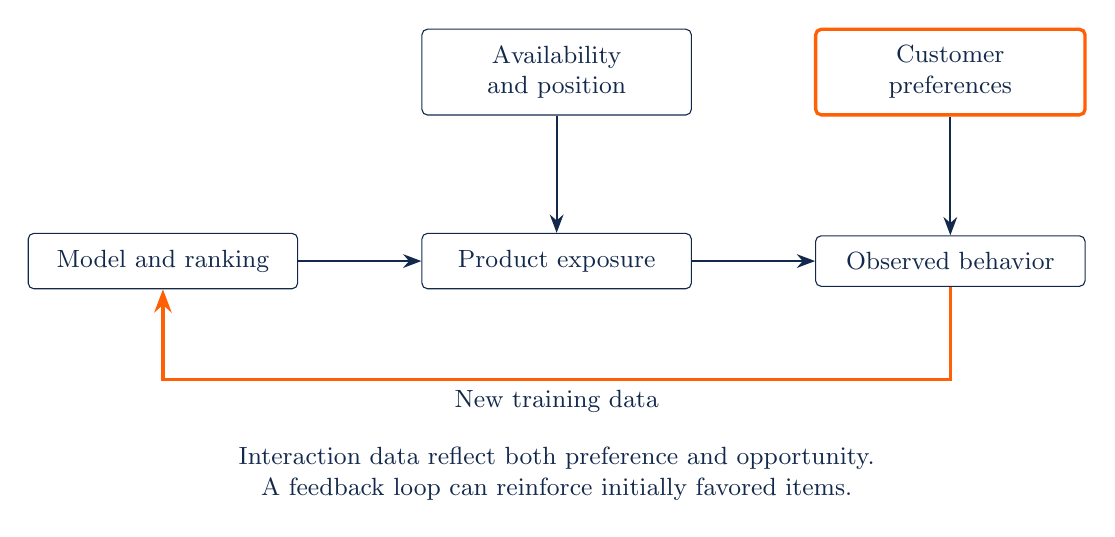
\begin{tikzpicture}
\node[box,text width=3cm] (m) at (0,0) {Model and ranking};
\node[box,text width=3cm] (e) at (5,0) {Product exposure};
\node[box,text width=3cm] (y) at (10,0) {Observed behavior};
\node[orangebox,text width=3cm] (p) at (10,2.4) {Customer preferences};
\node[box,text width=3cm] (a) at (5,2.4) {Availability and position};
\draw[edge] (m)--(e);\draw[edge] (e)--(y);\draw[edge] (p)--(y);\draw[edge] (a)--(e);
\draw[accent] (y.south)--(10,-1.5)--node[below] {New training data} (0,-1.5)--(m.south);
\node[align=center,text width=11cm] at (5,-2.7) {Interaction data reflect both preference and opportunity.\\A feedback loop can reinforce initially favored items.};
\end{tikzpicture}

\end{adjustbox}
\endgroup
\par\medskip
{\small The diagram describes a policy mechanism rather than an estimated effect.\par}
\note{A popularity loop can concentrate observation among already visible items. Randomized exploration or additional evaluation data can change what the system learns.

M8, Section 8.1, Marketing Analytics Lecture Notes. \url{../06_Lecture_Notes/modules/M08_Current_Topics_and_Integrated_Decisions.md}}
\end{frame}
\begin{frame}{The Evaluation Horizon Includes Learning}
\usebeamercolor[fg]{normal text}
\centering
\begingroup
\fontsize{11}{13.2}\selectfont
\def\small{\fontsize{10}{12}\selectfont}
\def\footnotesize{\fontsize{9}{11}\selectfont}
\def\scriptsize{\fontsize{8}{9.5}\selectfont}
\hyphenpenalty=10000
\begin{adjustbox}{max width=0.98\textwidth,max totalheight=0.65\textheight}
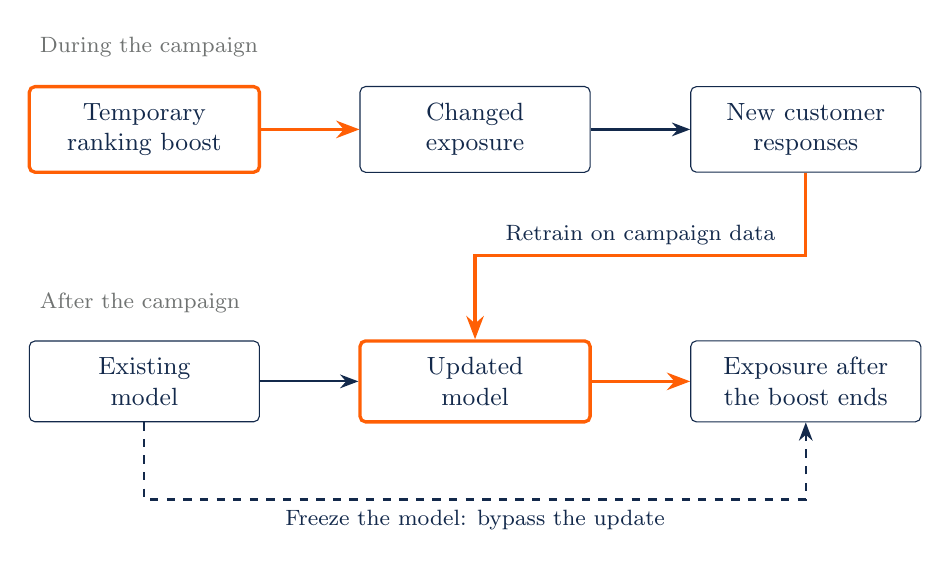
\begin{tikzpicture}
\node[orangebox,text width=2.5cm] (boost) at (0,0) {Temporary\\ranking boost};
\node[box,text width=2.5cm] (display) at (4.2,0) {Changed\\exposure};
\node[box,text width=2.5cm] (data) at (8.4,0) {New customer\\responses};
\draw[accent] (boost)--(display);
\draw[edge] (display)--(data);
\node[box,text width=2.5cm] (old) at (0,-3.2) {Existing\\model};
\node[orangebox,text width=2.5cm] (new) at (4.2,-3.2) {Updated\\model};
\node[box,text width=2.5cm] (future) at (8.4,-3.2) {Exposure after\\the boost ends};
\draw[edge] (old)--(new);
\draw[accent] (new)--(future);
\draw[accent] (data.south)--(8.4,-1.6)--node[above,font=\footnotesize] {Retrain on campaign data} (4.2,-1.6)--(new.north);
\draw[edge,dashed] (old.south)--(0,-4.7)--node[below,font=\footnotesize] {Freeze the model: bypass the update} (8.4,-4.7)--(future.south);
\node[anchor=west,font=\footnotesize,text=Storm] at (-1.45,1.05) {During the campaign};
\node[anchor=west,font=\footnotesize,text=Storm] at (-1.45,-2.2) {After the campaign};
\end{tikzpicture}

\end{adjustbox}
\endgroup
\par\medskip
{\small A temporary intervention can persist through subsequent model updates.\par}
\note{Freezing the model blocks the retraining channel but can leave direct changes in customer behavior. These policies require separate definitions and, where feasible, separate comparisons.

M8, Section 8.1.1, Marketing Analytics Lecture Notes. \url{../06_Lecture_Notes/modules/M08_Current_Topics_and_Integrated_Decisions.md}}
\end{frame}
\begin{frame}{Customer Goals and Platform Objectives}
\usebeamercolor[fg]{normal text}
\vfill
\begin{slidebullets}
\item Clicks reveal a response within an offered environment.
\item Considered preferences can differ from immediate engagement.
\item Measure satisfaction, unwanted repetition, and customer-stated goals.
\end{slidebullets}
\vfill
\note{A higher click count can coexist with regret or frustration. A system can combine behavior with explicit goals while recognizing that each measure has its own errors.

M8, Section 8.2.1, Marketing Analytics Lecture Notes. \url{../06_Lecture_Notes/modules/M08_Current_Topics_and_Integrated_Decisions.md}}
\end{frame}
\begin{frame}{A List Objective}
\usebeamercolor[fg]{normal text}
\noindent A list combines item relevance with category variety.
\medskip
\[
J(L)=\sum_{j\in L}s_j+\lambda K(L)
\]
\medskip
\noindent The variety weight $\lambda$ is expressed in the same units as the relevance score.
\note{A weighted sum requires a substantive choice of scales and tradeoffs. A customer replenishing a familiar basket may prefer a different weight from a customer seeking variety.

M8, Section 8.2, Marketing Analytics Lecture Notes. \url{../06_Lecture_Notes/modules/M08_Current_Topics_and_Integrated_Decisions.md}}
\end{frame}
\begin{frame}{Two Three-Item Lists}
\usebeamercolor[fg]{normal text}
\vfill
\centering
{\small\begin{tabular}{lrrr}
\toprule
List & Relevance & Categories & Value at 0.30 \\
\midrule
A, B, C & 2.50 & 2 & 3.10 \\
A, C, D & 2.30 & 3 & 3.20 \\
\bottomrule
\end{tabular}}
\par\medskip
Synthetic scores. The lists tie at a variety weight of 0.20.
\vfill
\note{A and B are coffee, C is tea, and D is fruit. The variety gain trades off against 0.20 of relevance. The values are imposed teaching scores.

M8, Section 8.2, Marketing Analytics Lecture Notes. \url{../06_Lecture_Notes/modules/M08_Current_Topics_and_Integrated_Decisions.md}}
\end{frame}
\begin{frame}{Model-Based and Experimental Evidence}
\usebeamercolor[fg]{normal text}
\vfill
\begin{slidebullets}
\item A fitted choice model can compare alternative recommenders.
\item A randomized perturbation can test predicted response patterns.
\item Engagement, retention, revenue, and welfare are distinct outcomes.
\end{slidebullets}
\vfill
\note{The Netflix study discussed in the notes uses a fitted choice model and an experimental check. Its replacement-recommender comparisons are model-based counterfactuals with specific exposure conditions.

M8, Section 8.1.2, Marketing Analytics Lecture Notes. \url{../06_Lecture_Notes/modules/M08_Current_Topics_and_Integrated_Decisions.md}}
\end{frame}
\begin{frame}{Marketing-Mix Modeling}
\usebeamercolor[fg]{normal text}
\vfill
\begin{slidebullets}
\item Weekly channel spending can have delayed effects.
\item Response can saturate at high exposure.
\item Spending decisions can respond to anticipated demand.
\end{slidebullets}
\vfill
\note{Trend, seasonality, promotions, and media can move together. A fitted media component requires an identification argument before it is interpreted as a causal contribution.

M8, Section 8.3, Marketing Analytics Lecture Notes. \url{../06_Lecture_Notes/modules/M08_Current_Topics_and_Integrated_Decisions.md}}
\end{frame}
\begin{frame}{Carryover}
\usebeamercolor[fg]{normal text}
\noindent A geometric accumulated-exposure measure retains earlier spending.
\medskip
\[
a_t=s_t+\rho a_{t-1},\qquad 0\leq\rho<1
\]
\medskip
\noindent A 100-unit pulse with $\rho=0.5$ gives 100, 50, 25, and 12.5 in successive periods.
\note{This definition is unnormalized. Under constant spending s, its long-run level is s divided by one minus rho. Coefficients must follow the implementation's normalization.

M8, Section 8.3, Marketing Analytics Lecture Notes. \url{../06_Lecture_Notes/modules/M08_Current_Topics_and_Integrated_Decisions.md}}
\end{frame}
\begin{frame}{Saturation and the Next Dollar}
\usebeamercolor[fg]{normal text}
\noindent A concave response has declining marginal contribution.
\medskip
\[
R(s)=A[1-\exp(-s/b)],\qquad R^{\prime}(s)=\frac{A}{b}\exp(-s/b)
\]
\medskip
\noindent Budget transfers depend on marginal response at the current allocation.
\note{Average response summarizes all earlier units of spending. The next small transfer depends on the local slope, with units of contribution per spending unit.

M8, Section 8.4, Marketing Analytics Lecture Notes. \url{../06_Lecture_Notes/modules/M08_Current_Topics_and_Integrated_Decisions.md}}
\end{frame}
\begin{frame}{Average and Marginal Returns Can Disagree}
\usebeamercolor[fg]{normal text}
\centering
\begingroup
\begin{adjustbox}{max width=0.98\textwidth,max totalheight=0.65\textheight}
% Original synthetic teaching figure; see corresponding module.
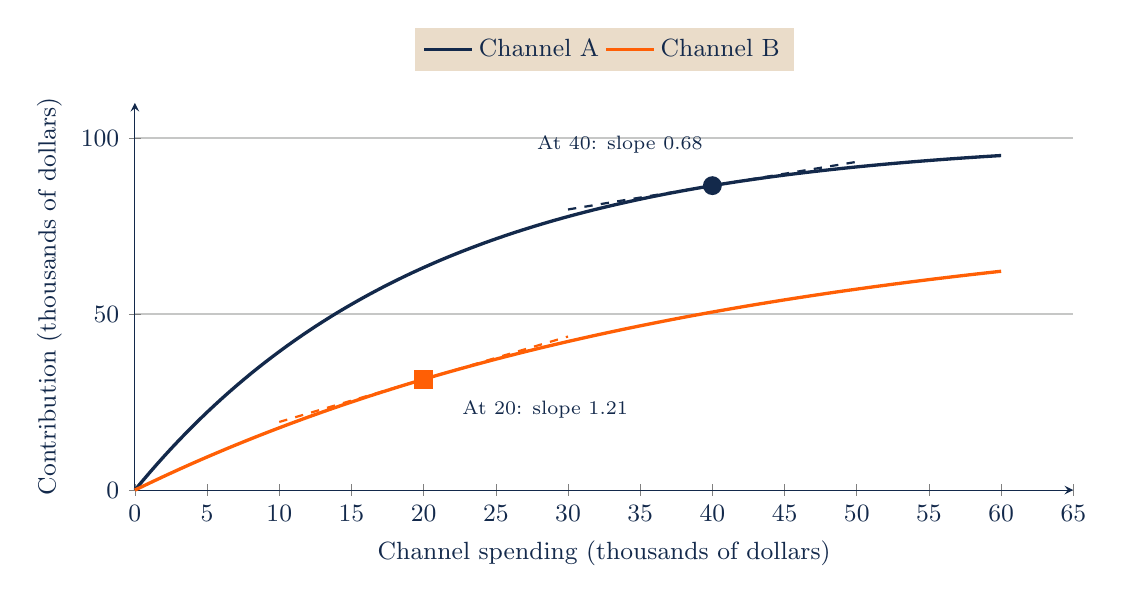
\begin{tikzpicture}
\begin{axis}[xmin=0,xmax=65,ymin=0,ymax=110,xlabel={Channel spending (thousands of dollars)},ylabel={Contribution (thousands of dollars)},legend style={at={(.5,1.08)},anchor=south,legend columns=2},ymajorgrids=true]
\addplot[IlliniBlue,very thick,domain=0:60,samples=120] {100*(1-exp(-x/20))};
\addplot[IlliniOrange,very thick,domain=0:60,samples=120] {80*(1-exp(-x/40))};
\legend{Channel A,Channel B}
\addplot[IlliniBlue,dashed,domain=30:50] {86.4665+.676676*(x-40)};
\addplot[IlliniOrange,dashed,domain=10:30] {31.4775+1.21306*(x-20)};
\addplot[only marks,mark=*,IlliniBlue,mark size=3pt] coordinates {(40,86.4665)};
\addplot[only marks,mark=square*,IlliniOrange,mark size=3pt] coordinates {(20,31.4775)};
\node[anchor=south east,font=\scriptsize] at (axis cs:40,93) {At 40: slope 0.68};
\node[anchor=north west,font=\scriptsize] at (axis cs:22,28) {At 20: slope 1.21};
\end{axis}
\end{tikzpicture}

\end{adjustbox}
\endgroup
\par\medskip
{\small Synthetic known response curves. Total spending is fixed at 60 thousand dollars.\par}
\note{The response curves are 100 times one minus exp(-sA/20) and 80 times one minus exp(-sB/40). The interior allocation equalizes marginal returns.

M8, Section 8.4, Marketing Analytics Lecture Notes. \url{../06_Lecture_Notes/modules/M08_Current_Topics_and_Integrated_Decisions.md}}
\end{frame}
\begin{frame}[fragile]{The Fixed-Budget Optimum}
\usebeamercolor[fg]{normal text}
\noindent Solve equal marginal returns for the imposed curves.
\begin{lstlisting}
from math import exp, log
budget = 60
a = (log(2.5) + budget/40) / (1/20 + 1/40)
b = budget - a
ma = 5 * exp(-a/20)
mb = 2 * exp(-b/40)
assert abs(ma-mb) < 1e-12
\end{lstlisting}
{\small The allocation is about 32.22 to A and 27.78 to B, in thousands of dollars.\par}
\note{The closed-form result applies to these known concave curves and an interior fixed-budget optimum. Different constraints or uncertain response functions require a revised calculation.

M8, Section 8.4, Marketing Analytics Lecture Notes. \url{../06_Lecture_Notes/modules/M08_Current_Topics_and_Integrated_Decisions.md}}
\end{frame}
\begin{frame}{Coding Exercise: A Policy Objective}
\usebeamercolor[fg]{normal text}
\vfill
\begin{slidebullets}
\item Enumerate three-item lists at several variety weights.
\item Solve and independently grid-check the fixed-budget allocation.
\item Report the assumptions that change the preferred action.
\end{slidebullets}
\vfill
\note{Run ../03\_Data\_and\_Code/Lecture\_Examples/session\_examples.py S13. A grid check verifies the numerical optimum within its resolution. It does not establish the imposed response curves as causal estimates.

M8, Section 8.10, Marketing Analytics Lecture Notes. \url{../06_Lecture_Notes/modules/M08_Current_Topics_and_Integrated_Decisions.md}}
\end{frame}
\begin{frame}{Attention and the Optimization Target}
\usebeamercolor[fg]{normal text}
\vfill
\begin{slidebullets}
\item A free service can require customer time and attention.
\item More exposure can benefit advertisers while burdening customers.
\item Evaluate voluntary use and customer outcomes alongside engagement.
\end{slidebullets}
\vfill
\note{Tim Wu's Blind Spot discusses attention markets and the difficulty of analyzing exchanges without a monetary user price. A course application should measure time, control, and value rather than equate engagement with welfare.

Tim Wu, Blind Spot: The Attention Economy and the Law (2019). \url{https://scholarship.law.columbia.edu/faculty_scholarship/2029/}}
\end{frame}
\begin{frame}{Policy Discussion}
\usebeamercolor[fg]{normal text}
\vfill
\begin{slidebullets}
\item What changes when the recommender learns during the experiment?
\item Which outcome measures the customer's stated goal?
\item How much uncertainty in response slopes would change the budget?
\end{slidebullets}
\vfill
\note{A robust decision states the learning rule, target outcome, and support for the response function. The best numerical optimizer cannot supply those definitions.

M8, Section 8.7, Marketing Analytics Lecture Notes. \url{../06_Lecture_Notes/modules/M08_Current_Topics_and_Integrated_Decisions.md}}
\end{frame}
\end{document}
